\documentclass[12pt]{article}
\usepackage{multicol}
\usepackage[shortlabels]{enumitem}
\usepackage{tikz}
\usepackage{tikz-qtree}
\begin{document}
\title{Linguistics 20, Homework 6}
\date{May 13th, 2019}
\author{Michael Wu\\UID: 404751542\\TA: Eleanor Glewwe\\Discussion 1F Friday 9:00-9:50 AM}
\maketitle

\section*{Chapter 5, Problem 3}

\tikzset{level distance = 0.8cm}
\begin{multicols}{2}
    \begin{enumerate}[a)]
        \item the zoo
        \begin{center}
            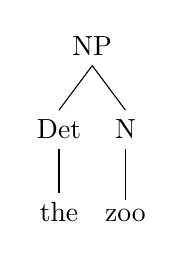
\begin{tikzpicture}
                \Tree [.NP [.Det the ] [.N zoo ] ]
            \end{tikzpicture}
        \end{center}
        \item always try
        \begin{center}
            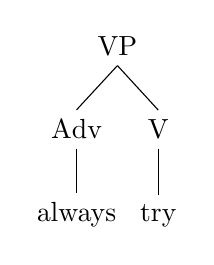
\begin{tikzpicture}
                \Tree [.VP [.Adv always ] [.V try ] ]
            \end{tikzpicture}
        \end{center}
        \item so witty
        \begin{center}
            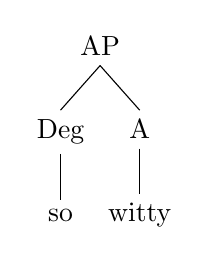
\begin{tikzpicture}
                \Tree [.AP [.Deg so ] [.A witty ] ]
            \end{tikzpicture}
        \end{center}
        \item perhaps pass
        \begin{center}
            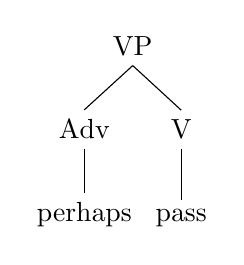
\begin{tikzpicture}
                \Tree [.VP [.Adv perhaps ] [.V pass ] ]
            \end{tikzpicture}
        \end{center}
        \item less bleak
        \begin{center}
            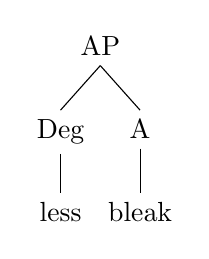
\begin{tikzpicture}
                \Tree [.AP [.Deg less ] [.A bleak ] ]
            \end{tikzpicture}
        \end{center}
        \item this house
        \begin{center}
            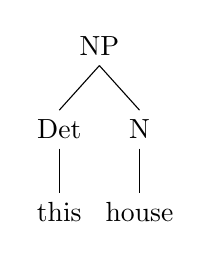
\begin{tikzpicture}
                \Tree [.NP [.Det this ] [.N house ] ]
            \end{tikzpicture}
        \end{center}
        \item very competent
        \begin{center}
            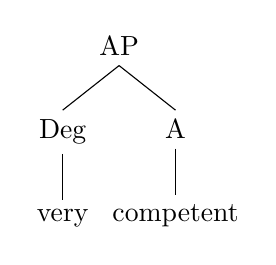
\begin{tikzpicture}
                \Tree [.AP [.Deg very ] [.A competent ] ]
            \end{tikzpicture}
        \end{center}
        \item quite cheap
        \begin{center}
            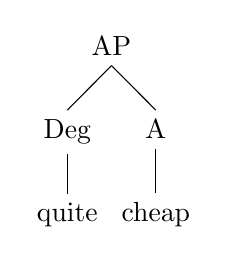
\begin{tikzpicture}
                \Tree [.AP [.Deg quite ] [.A cheap ] ]
            \end{tikzpicture}
        \end{center}
        \item never surrender
        \begin{center}
            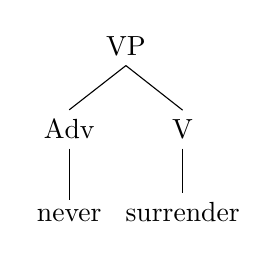
\begin{tikzpicture}
                \Tree [.VP [.Adv never ] [.V surrender ] ]
            \end{tikzpicture}
        \end{center}
        \item those books
        \begin{center}
            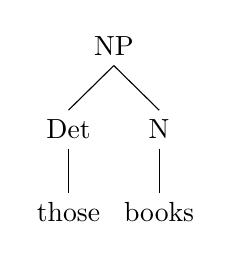
\begin{tikzpicture}
                \Tree [.NP [.Det those ] [.N books ] ]
            \end{tikzpicture}
        \end{center}
    \end{enumerate}
\end{multicols}

\section*{Chapter 5, Problem 4}

\tikzset{level distance = 1cm, sibling distance = 0cm}
\begin{multicols}{2}
    \begin{enumerate}[a)]
        \item into the house
        \begin{center}
            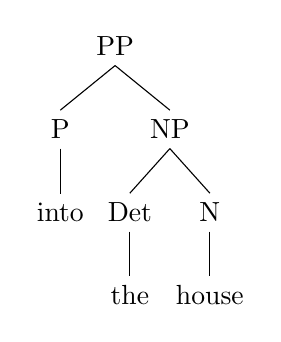
\begin{tikzpicture}
                \Tree [.PP [.P into ] [.NP [.Det the ] [.N house ] ] ]
            \end{tikzpicture}
        \end{center}
        \item fixed the printer
        \begin{center}
            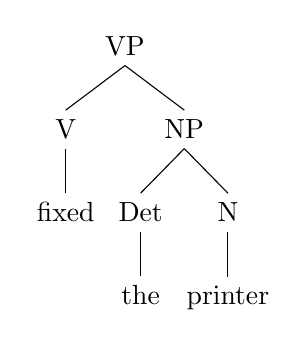
\begin{tikzpicture}
                \Tree [.VP [.V fixed ] [.NP [.Det the ] [.N printer ] ] ]
            \end{tikzpicture}
        \end{center}
        \tikzset{level distance = 0.8cm}
        \item full of mistakes
        \begin{center}
            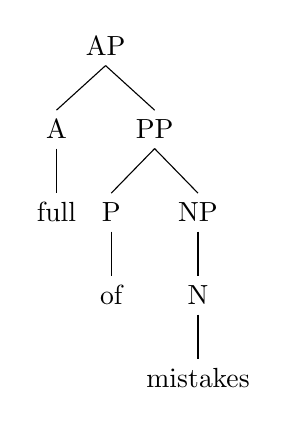
\begin{tikzpicture}
                \Tree [.AP [.A full ] [.PP [.P of ] [.NP [.N mistakes ] ] ] ]
            \end{tikzpicture}
        \end{center}
        \item more toward the window
        \begin{center}
            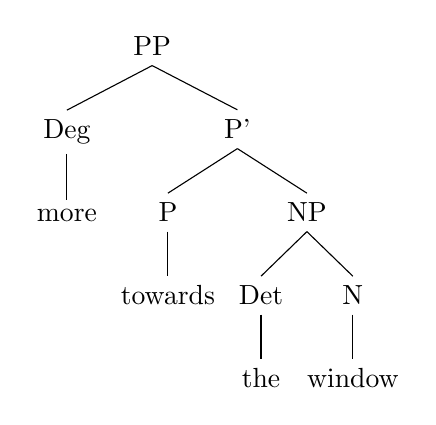
\begin{tikzpicture}
                \Tree [.PP [.Deg more ] [.P' [.P towards ] [.NP [.Det the ] [.N window ] ] ] ]
            \end{tikzpicture}
        \end{center}
        \tikzset{level distance = 0.7cm, every picture/.style = {scale=0.9}}
        \item a film about pollution
        \begin{center}
            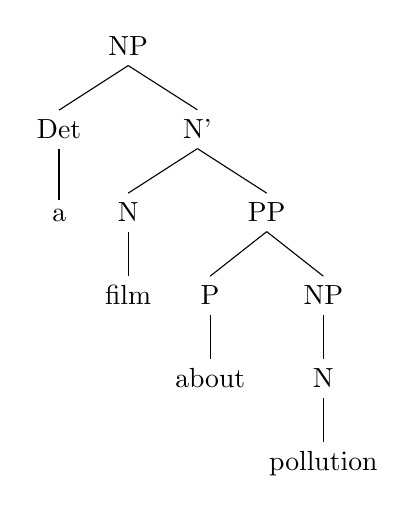
\begin{tikzpicture}
                \Tree [.NP [.Det a ] [.N' [.N film ] [.PP [.P about ] [.NP [.N pollution ] ] ] ] ]
            \end{tikzpicture}
        \end{center}
        \item always study this material
        \begin{center}
            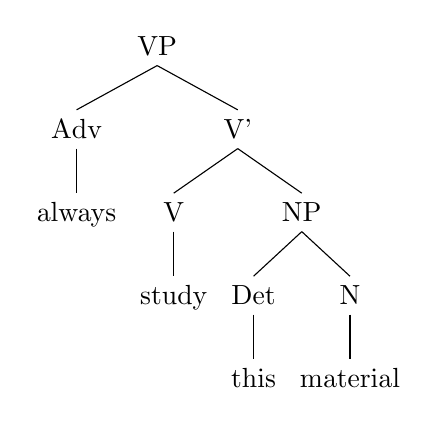
\begin{tikzpicture}
                \Tree [.VP [.Adv always ] [.V' [.V study ] [.NP [.Det this ] [.N material ] ] ] ]
            \end{tikzpicture}
        \end{center}
        \item perhaps earn the money
        \begin{center}
            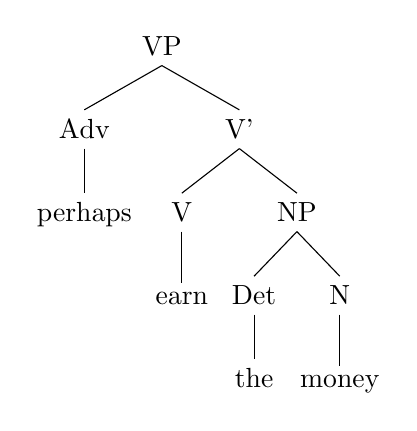
\begin{tikzpicture}
                \Tree [.VP [.Adv perhaps ] [.V' [.V earn ] [.NP [.Det the ] [.N money ] ] ] ]
            \end{tikzpicture}
        \end{center}
        \item that argument with Owen
        \vspace{-0.29cm}
        \begin{center}
            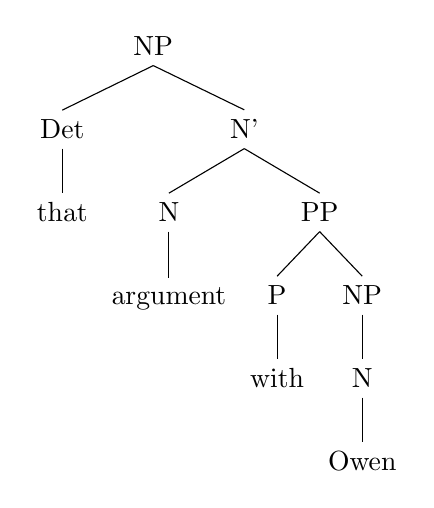
\begin{tikzpicture}
                \Tree [.NP [.Det that ] [.N' [.N argument ] [.PP [.P with ] [.NP [.N Owen ] ] ] ] ]
            \end{tikzpicture}
        \end{center}
        \vspace{-0.29cm}
        \item the success of the program
        \begin{center}
            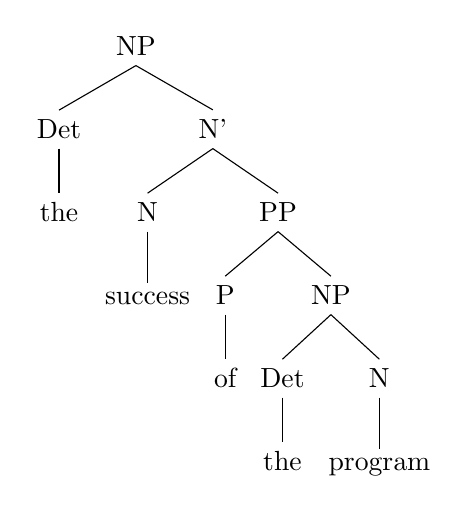
\begin{tikzpicture}
                \Tree [.NP [.Det the ] [.N' [.N success ] [.PP [.P of ] [.NP [.Det the ] [.N program ] ] ] ] ] ]
            \end{tikzpicture}
        \end{center}
        \vfill\null
    \end{enumerate}
\end{multicols}

\section*{Chapter 5, Problem 5}

\tikzset{level distance = 0.7cm, every picture/.style = {scale=0.55}}
\begin{multicols}{2}
    \begin{enumerate}[a)]
        \item Those guests should leave.
        \begin{center}
            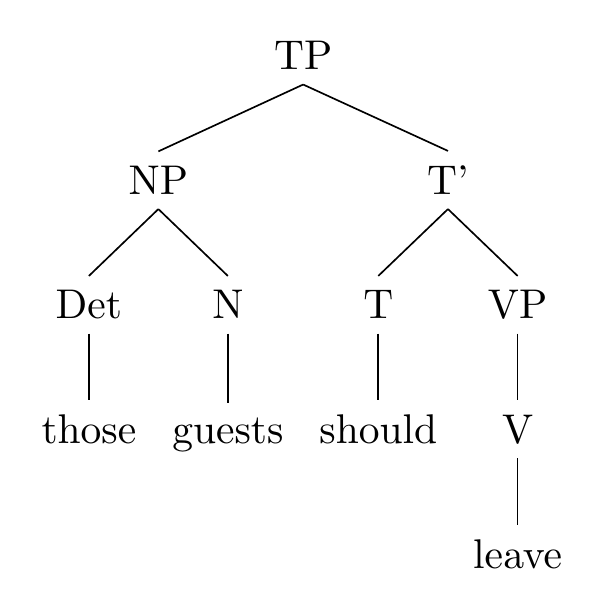
\begin{tikzpicture}[scale=1.5]
                \Tree [.TP [.NP [.Det those ] [.N guests ] ] [.T' [.T should ] [.VP [.V leave ] ] ] ]
            \end{tikzpicture}
        \end{center}
        \item Maria never ate a brownie.
        \begin{center}
            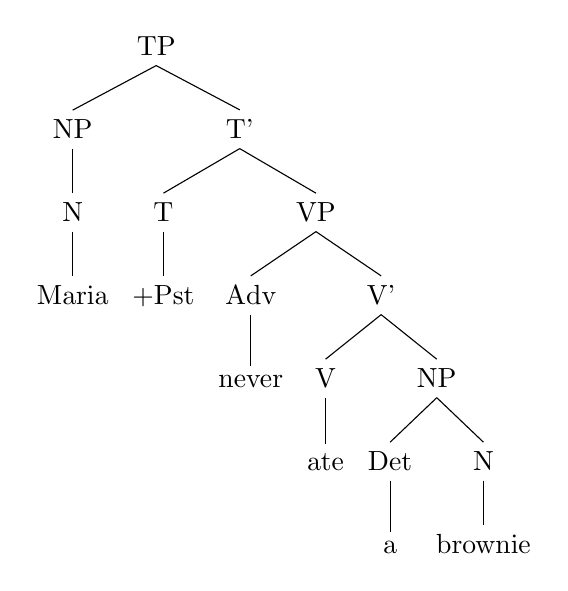
\begin{tikzpicture}
                \Tree [.TP [.NP [.N Maria ] ] [.T' [.T +Pst ] [.VP [.Adv never ] [.V' [.V ate ] [.NP [.Det a ] [.N brownie ] ] ] ] ] ]
            \end{tikzpicture}
        \end{center}
        \item That shelf will fall.
        \begin{center}
            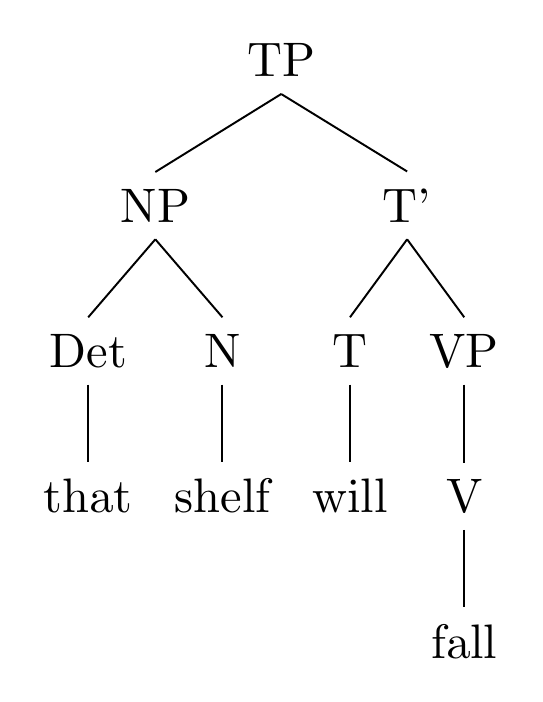
\begin{tikzpicture}[scale=1.75]
                \Tree [.TP [.NP [.Det that ] [.N shelf ] ] [.T' [.T will ] [.VP [.V fall ] ] ] ]
            \end{tikzpicture}
        \end{center}
        \item The glass broke.
        \begin{center}
            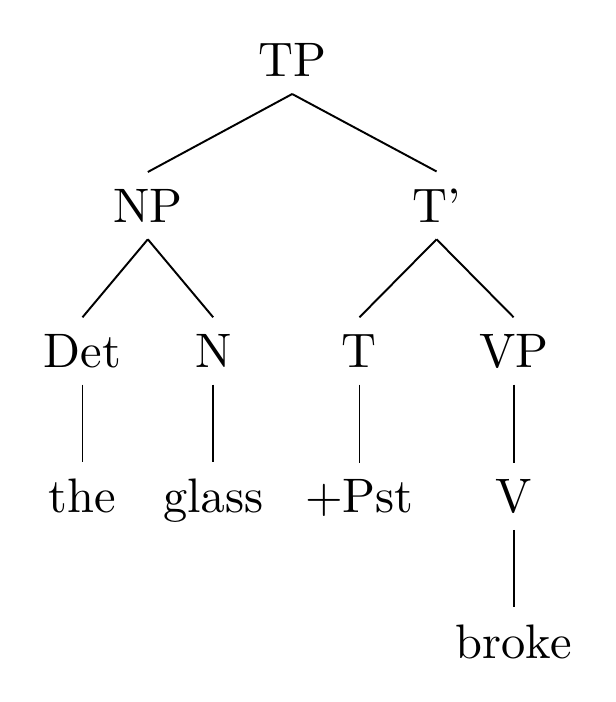
\begin{tikzpicture}[scale=1.75]
                \Tree [.TP [.NP [.Det the ] [.N glass ] ] [.T' [.T +Pst ] [.VP [.V broke ] ] ] ]
            \end{tikzpicture}
        \end{center}
        \item The student lost the debate.
        \begin{center}
            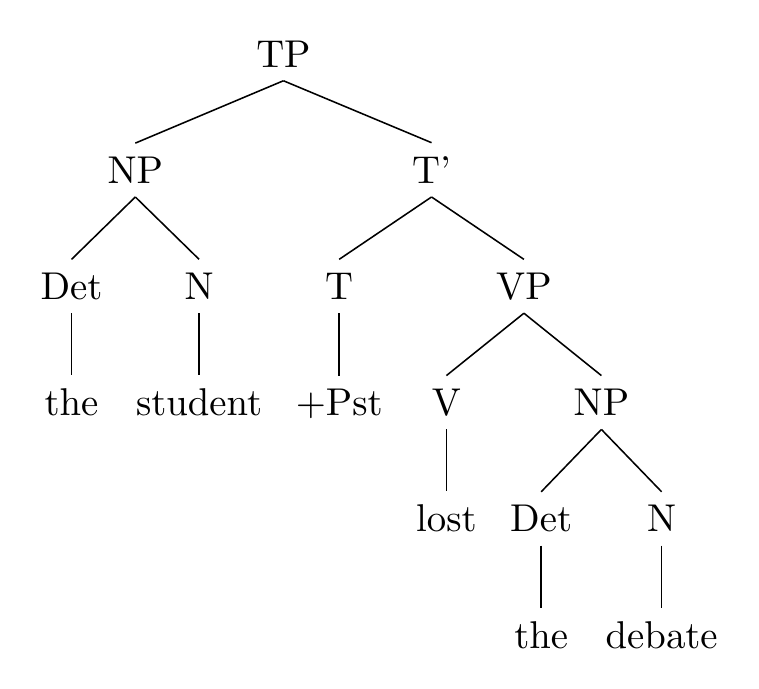
\begin{tikzpicture}[scale=1.4]
                \Tree [.TP [.NP [.Det the ] [.N student ] ] [.T' [.T +Pst ] [.VP [.V lost ] [.NP [.Det the ] [.N debate ] ] ] ] ]
            \end{tikzpicture}
        \end{center}
        \item The manager may offer a raise.
        \begin{center}
            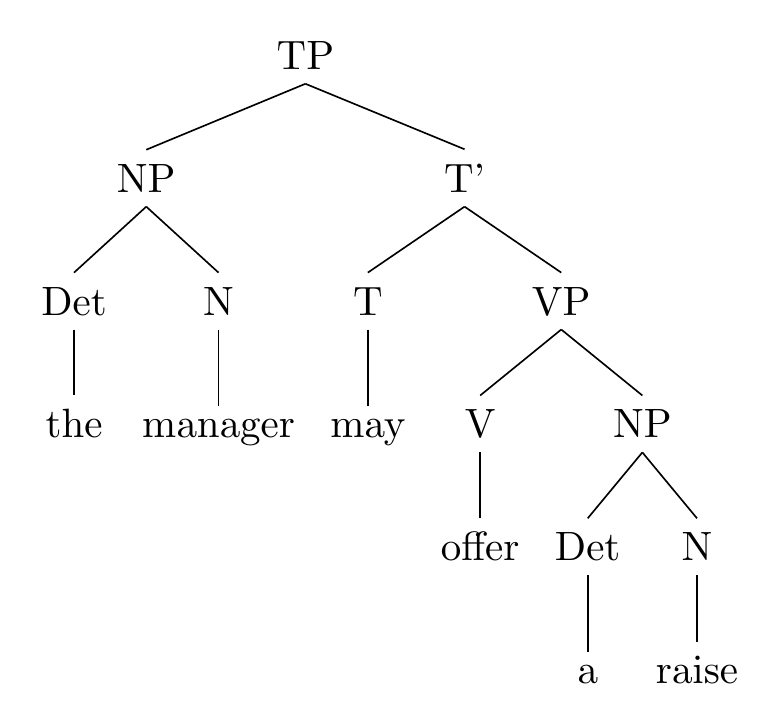
\begin{tikzpicture}[scale=1.48]
                \Tree [.TP [.NP [.Det the ] [.N manager ] ] [.T' [.T may ] [.VP [.V offer ] [.NP [.Det a ] [.N raise ] ] ] ] ]
            \end{tikzpicture}
        \end{center}
        \vfill\null
        \columnbreak
        \item The judge never jails shop\-lifters.
        \begin{center}
            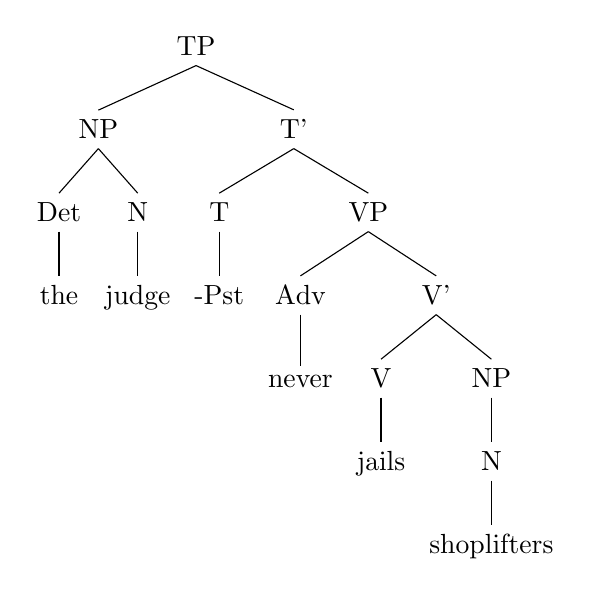
\begin{tikzpicture}
                \Tree [.TP [.NP [.Det the ] [.N judge ] ] [.T' [.T -Pst ] [.VP [.Adv never ] [.V' [.V jails ] [.NP [.N shoplifters ] ] ] ] ] ]
            \end{tikzpicture}
        \end{center}
        \item The teacher often organized a discussion.
        \begin{center}
            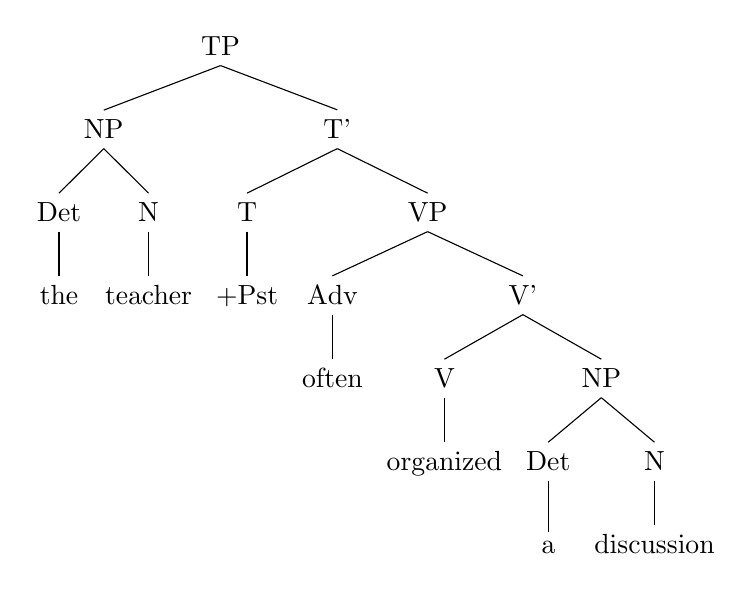
\begin{tikzpicture}
                \Tree [.TP [.NP [.Det the ] [.N teacher ] ] [.T' [.T +Pst ] [.VP [.Adv often ] [.V' [.V organized ] [.NP [.Det a ] [.N discussion ] ] ] ] ] ]
            \end{tikzpicture}
        \end{center}
        \item A psychic will speak to this group.
         \begin{center}
            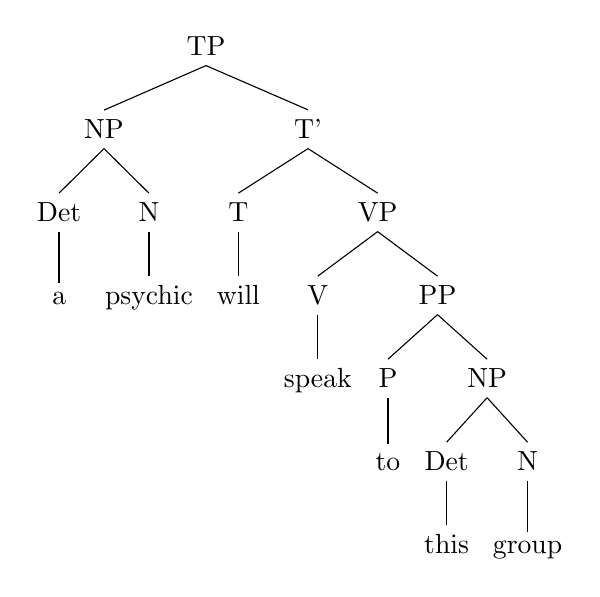
\begin{tikzpicture}
                \Tree [.TP [.NP [.Det a ] [.N psychic ] ] [.T' [.T will ] [.VP [.V speak ] [.PP [.P to ] [.NP [.Det this ] [.N group ] ] ] ] ] ]
            \end{tikzpicture}
        \end{center}
        \item Marianne could become quite fond of Larry.
         \begin{center}
            \begin{tikzpicture}
                \Tree [.TP [.NP [.N Marianne ] ] [.T' [.T could ] [.VP [.V become ] [.AP [.Deg quite ] [.A' [.A fond ] [.PP [.P of ] [.NP [.N Larry ] ] ] ] ] ] ] ]
            \end{tikzpicture}
        \end{center}
    \end{enumerate}
\end{multicols}

\section*{Chapter 5, Problem 6}

\begin{enumerate}[a)]
    \item {[\textsubscript{NP} The news] upset the entire family. [\textsubscript{NP} It] upset the entire family. This is a constituent.}
    \item They hid [\textsubscript{PP} in the cave]. They hid [\textsubscript{PP} under it]. This is a constituent.
    \item The [computer was very] expensive. This is not a constituent, as it does not fit any form that follows the X' schema and cannot be replaced.
    \item {[\textsubscript{NP} The houses] will be rebuilt. [\textsubscript{NP} It] will be rebuilt. This is a constituent.}
    \item Jane will [\textsubscript{VP} leave town]. Jane will [\textsubscript{VP} go]. This is a constituent.
    \item The goslings [swam across] the lake. This is not a constituent, since the X' schema requires that the verb phrase includes ``the lake''.
    Although ``swam across'' could be a verb phrase by itself, its position within the sentence means we cannot separate it and replace it with any other verb phrase.
\end{enumerate}

\section*{Chapter 5, Problem 7}

\begin{enumerate}[a)]
    \item We ate our lunch [\textsubscript{PP} near the river bank]. [\textsubscript{PP} Near the river bank], we ate our lunch. This is a constituent.
    \item Steve looked [up the number] in the book. This is not a constituent, as we cannot move it anywhere that makes sense. The words ``looked up'' need to stay together.
    \item The [island has been] flooded. This is not a constituent, as we cannot move it anywhere that makes sense. The words ``has been'' should be grouped with the verb ``flooded''.
    \item I love [peanut butter and bacon sandwiches]. Although this phrase makes sense as a noun phrase, the movement test does not work since we cannot move it anywhere that makes sense.
    \item The environmental [movement is gaining momentum]. This is not a constituent, as we cannot move it anywhere that makes sense.
\end{enumerate}

\end{document}